% Please make sure you insert your
% data according to the instructions in PoSauthmanual.pdf
\documentclass[a4paper,11pt]{article}
\usepackage{pos}

\usepackage{mciteplus}

\title{Finite temperature and $\delta$-regime in the Schwinger model}
%% \ShortTitle{Short Title for header}

\author*[a]{Ivan Hip}
\author[b]{Jaime Fabián Nieto Castellanos}
\author[c]{Wolfgang Bietenholz}

\affiliation[a]{ Faculty of Geotechnical Engineering, University of Zagreb \\
  Hallerova aleja 7, 42000 Varaždin, Croatia}

\affiliation[b]{
Facultad de Ciencias, Universidad Nacional Autónoma de México \\A.P. 70-542, C.P. 04510 Ciudad de México, Mexico}

\affiliation[c]{
Instituto de Ciencias Nucleares, Universidad Nacional Autónoma de México \\
A.P. 70-543, C.P. 04510 Ciudad de México, Mexico}

\emailAdd{ivan.hip@gfv.unizg.hr}
\emailAdd{jafanica@ciencias.unam.mx}
\emailAdd{wolbi@nucleares.unam.mx}

\abstract{
The Schwinger model is often used as a testbed for conceptual and numerical
approaches in lattice field theory. Nevertheless, some of the rich physical
properties of the model in anisotropic volumes have not yet been tested.
For the multi-flavor finite temperature Schwinger model there is an
approximate solution by Hosotani et al. based on bosonization. We perform
thorough comparisons with the lattice results and check the validity and
limitations of the Hosotani approach. By inverting the physical interpretation
of the coordinates we explore the delta-regime and measure the dependence of
the pion mass on the spatial size at zero temperature. Our results confirm
universal features of theoretical predictions by Leutwyler, Hasenfratz and
Niedermayer and enable the computation of the Schwinger model counterpart of
pion decay constant. This is further compared with the 2d version of the
Witten-Veneziano formula.}

\FullConference{%
 The 38th International Symposium on Lattice Field Theory, LATTICE2021
  26th-30th July, 2021
  Zoom/Gather@Massachusetts Institute of Technology
}

%% \tableofcontents

\begin{document}
\maketitle


\section{Introduction}

%\begin{frame}{Schwinger model}
  \begin{itemize}
    \item introduced by [Schwinger, 1961]\cite{Schwinger1962a}
      \textit{two-dimensional quantum electrodynamics}
      --- fermions coupled to Abelian gauge field 
    \item simple example for chiral anomaly, topology, confinement
    \item often used as a testbed for conceptual and numerical
      approaches in lattice field theory
    \item nevertheless, some of the rich physical properties of
      the model in anisotropic volumes have not yet been tested:
  \end{itemize}
  \begin{description}
    \item[Finite temperature]:
      Hosotani et al. approximate solution has not been compared with the lattice
      simulation results
    \item[$\delta$-regime]: conjecture for the residual pion mass
  \end{description}
%\end{frame}

%\begin{frame}{$N$-flavor Schwinger model}
  \begin{itemize}
    \item massless case has analytic solution
      [Belvedere et al., 1979]\cite{Belvedere1979}
    \item $N - 1$ massless bosons ("pions")
    \item one massive boson ("eta")
      \[
        m_\eta^2 = N\,\frac{g^2}{\pi}
      \]
      where $g$ is the gauge coupling
    \item massive case (fermion mass $m > 0$) has no exact solution
    \item semiclassical prediction at infinite volume [Hetrick, Hosotani and
      Iso, 1995]\cite{Hetrick1995}
      \[
        m_\pi = \left(4e^{2\gamma}\sqrt{\frac{2}{\pi}}\right)
          (m^2 g)^{1/3} = 2.1633...(m^2 g)^{1/3}
      \]        
  \end{itemize}
%\end{frame}

  
\section{Finite temperature}

%\begin{frame}{Finite temperature - Hosotani approximate solution}
  \begin{itemize}
    \item approximate solution by Hosotani et al.\cite{Hetrick1996}
      based on bosonization
    \item finite temperature massive Schwinger model reduced to
      quantum mechanical system with $N - 1$ degrees of freedom
    \item set of nonlinear equations valid when
      \[
        m \ll m_\eta
      \]
    \item boson masses can be computed by solving this set of 
      equations in a self-consistent way
    \item we compare the Hosotani predictions for two flavors
      with HMC simulation results (Wilson fermions --- fermion mass
      $m$ is measured on the lattice by the PCAC relation)
  \end{itemize}
  %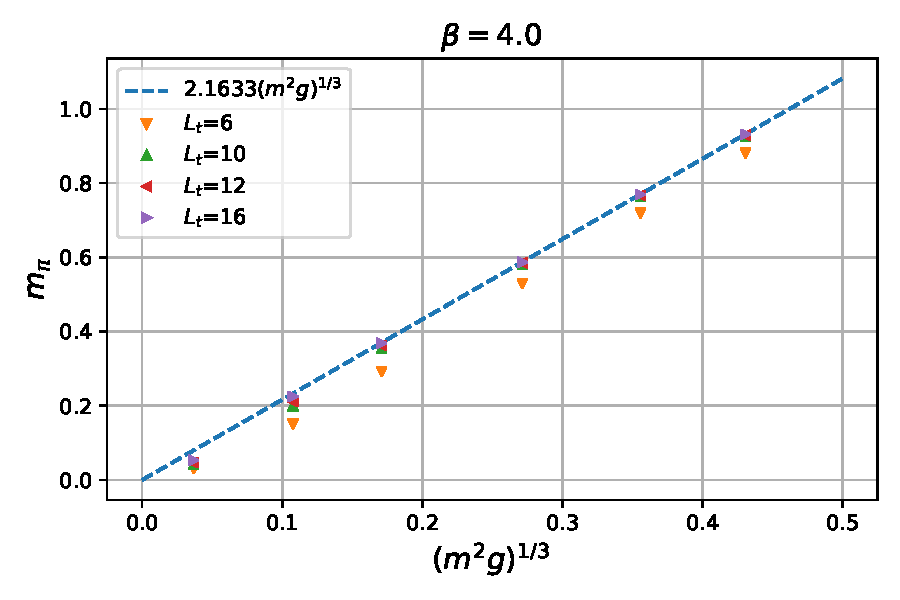
\includegraphics[width=1\textwidth]{figs/FiniteTMPiHos}
%\end{frame}

%\begin{frame}{Pion mass - Hosotani vs. lattice simulation}
\begin{figure}
  \includegraphics[width=1\textwidth]{figs/MPi64x10vsMFiniteT_Pt2}
  \caption{Pion mass as a function of quark mass.}
\end{figure}
%\end{frame}

%\begin{frame}{Eta mass - Hosotani vs. lattice simulation}
\begin{figure}
  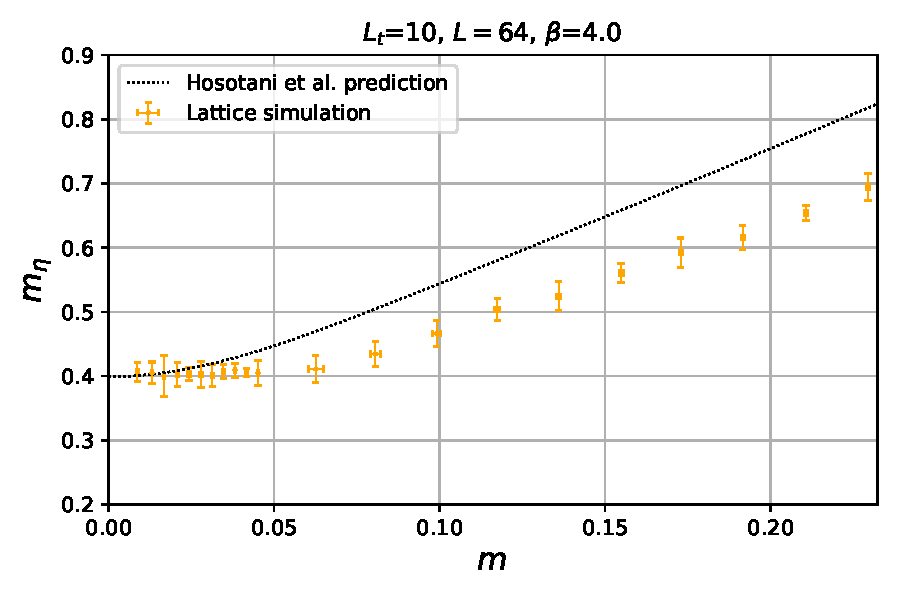
\includegraphics[width=1\textwidth]{figs/Meta64x10FiniteT_Pt3}
  \caption{Eta mass as a function of quark mass.}
\end{figure}
%\end{frame}


\section{\texorpdfstring{$\delta$}{d}-regime}

\{HIP: Wolfgang would probably like to cite \cite{Bietenholz2010} ;-)\}

%\begin{frame}{$\delta$-regime}
  \begin{itemize}
    \item spatial volume is small compared to the correlation
      length
      \[
        \xi = m_\pi^{-1}
      \]
      but the Euclidean time extent is large
      \[
        L_t\gg \xi \gtrsim L
      \]
    \item the system is quasi one dimensional - approximation by
      quantum mechanical rotor [Leutwyler, 1987\cite{Leutwyler1987}
    \item pion has \textbf{\textit{residual mass}}
      \[
        m_\pi^R = \frac{{\cal N} - 1}{2\Theta}
      \]
    \item ${\cal N} - 1$ is the number of pions and $\Theta$ is the moment of
      inertia
  \end{itemize}
%\end{frame}

%\begin{frame}{Residual pion mass plateau}
\begin{figure}
  \begin{tabular}{cc}
    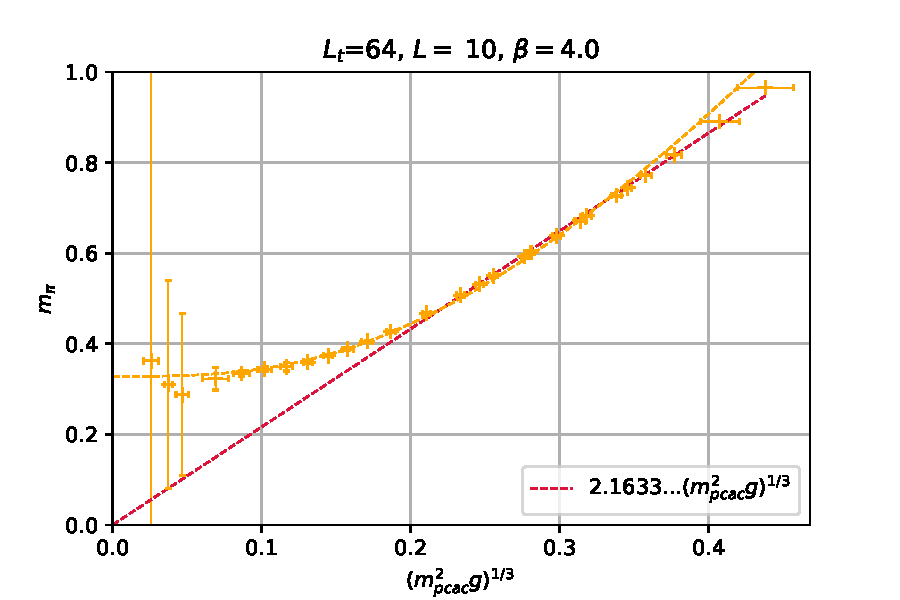
\includegraphics[width=0.5\textwidth]{figs/Mpi10x64} &
    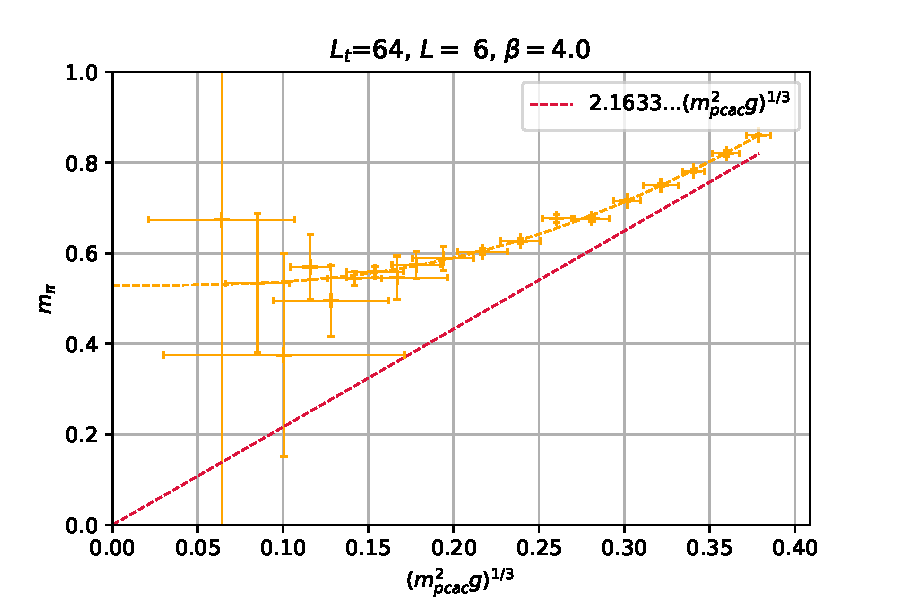
\includegraphics[width=0.5\textwidth]{figs/Mpi6x64Pt10}
  \end{tabular}
  \caption{Residual pion mass plateaus for two different spatial volumes.}
\end{figure}
%\end{frame}

%\begin{frame}{Conjecture}
  \begin{itemize}
    \item {}[Hasenfratz and Niedermayer, 1993]\cite{Hasenfratz1993} computed
      $\Theta$ up to next-to-leading order, for a general dimension $d > 2$
      \[
        \Theta = F_\pi^2 L^{d-1} \left[1 +
          \frac{{\cal N} - 2}{4\pi F_\pi^2 L^{d-2}}
          \left(2\frac{d - 1}{d - 2} + ...\right) \right]
      \]
    \item for ${\cal N} = 2$ we ignore the next to leading term despite
      the division by $d - 2$,
      so we just consider the leading term
      \[
        m_\pi^R \simeq \frac{{\cal N} - 1}{2F_\pi^2 L}
      \]
    \item we verify the relation $m_\pi^R \propto 1 / L$ with
      simulation data and extract the value of pion decay
      constant $F_\pi$
  \end{itemize}
%\end{frame}

%\begin{frame}{1 / L confirmed by lattice simulation}
\begin{figure}
  \begin{tabular}{cc}
    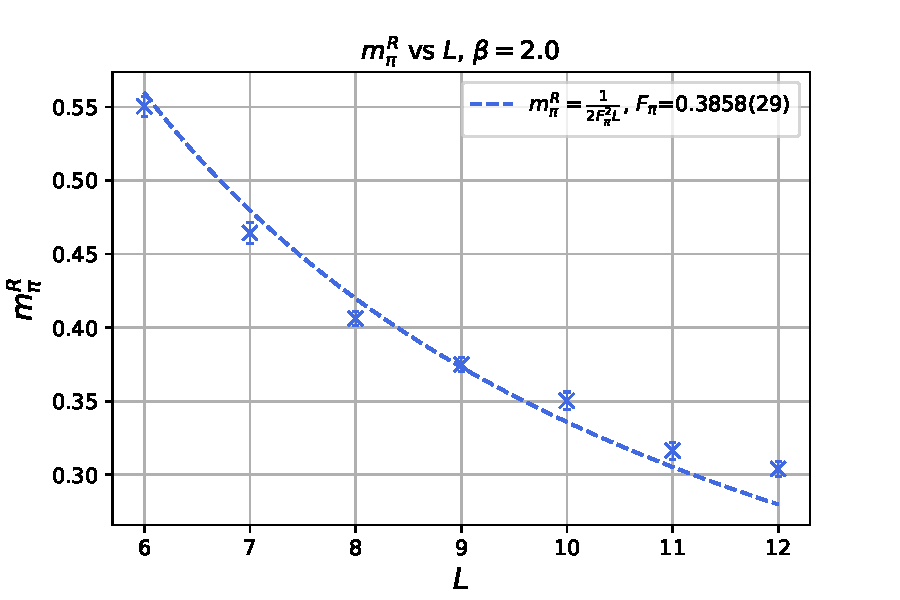
\includegraphics[width=0.5\textwidth]{figs/ResMpiBeta2} &
    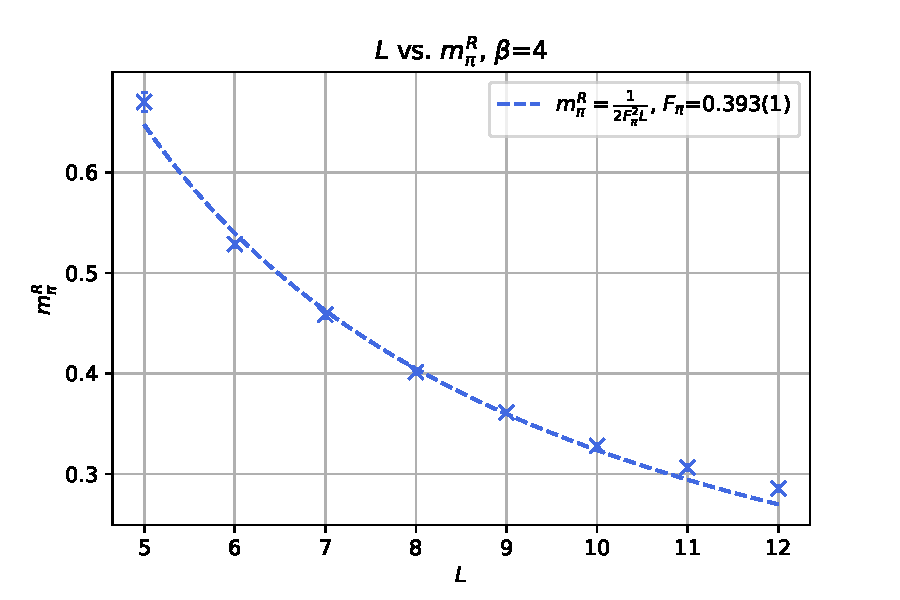
\includegraphics[width=0.5\textwidth]{figs/ResMpiBeta4} \\
    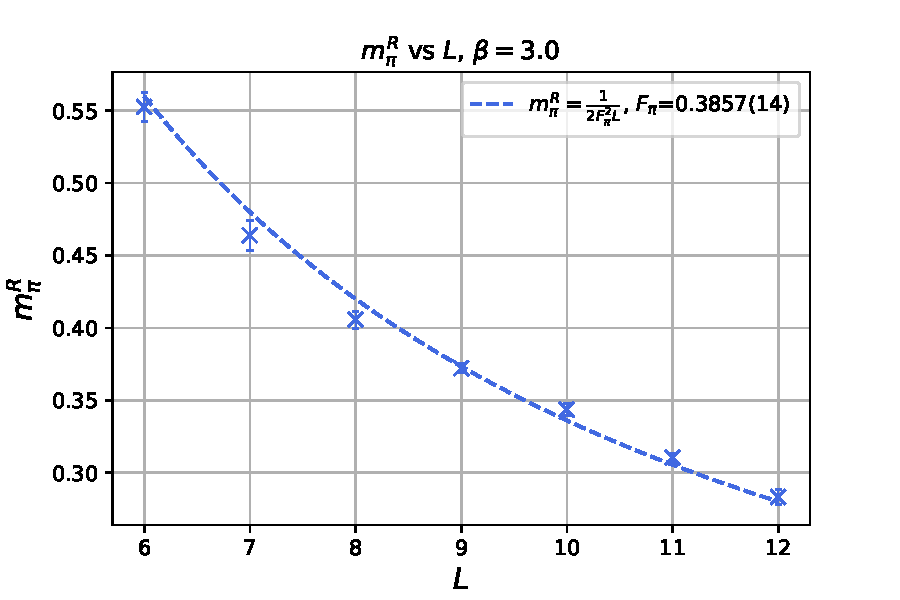
\includegraphics[width=0.5\textwidth]{figs/ResMpiBeta3}
  \end{tabular}
  \caption{1 / L confirmed by lattice simulation ($\beta = 5.0$ still missing).}
\end{figure}

      \begin{center} 
	    \begin{tabular}{c c c c}
	      $\beta$ & $F_\pi$ \\
	      \hline
	      2.0 & 0.3858(29) \\
	      \hline
	      3.0 & 0.3857(14) \\
	      \hline
	      4.0 & 0.3868(13) \\
	    \end{tabular}
        \[
      	  F_\pi = 0.386(2)
        \]
      \end{center}	 
%\end{frame}


\section{Witten-Veneziano}

\{HIP: here we probably should cite \cite{Witten1979, *Veneziano1979}\}

%\begin{frame}{Witten-Veneziano formula for Schwinger model}
  \begin{itemize}
    \item in the chiral $N$-flavor Schwinger model the
      Witten-Veneziano formula is simplified to [Seiler and
      Stamatescu, 1987]\cite{Seiler1987}
      \textit{\{HIP: this Seiler and Stamatescu paper from 1987 is unpublished
        and exists only as a KEK scan --- it has just few lines 
        about 1-flavor Schwinger model, so for N-flavor SM makes 
        probably more sense to cite \cite{Gattringer1994}\}}
      \[
        m_\eta^2 = \frac{2N}{F_\eta^2}\chi_T^{que}
      \]
    \item $m_\eta$ in the chiral limit is known analytically
      [Belvedere et al., 1979]\cite{Belvedere1979}
      \[
        m_\eta^2 = \frac{N}{\pi\beta}
      \]
    \item continuum prediction for $\chi_T^{que}$
      [Seiler and Stamatescu, 1987]
      \[
        \beta\chi_T^{que} = \frac{1}{4\pi^2}
      \]
  \end{itemize}
%\end{frame}

%\begin{frame}{Quenched topological susceptibility on the lattice}
  \begin{itemize}
    \item {} [Bardeen et al., 1998]\cite{Bardeen1998}
      were able to analytically
      compute $\chi_T^{que}$ on the lattice
      \[
        \beta\chi_T^{que} = \frac{I_1(\beta)}{4 \pi^2 I_0(\beta)}
      \]
      \setlength{\abovedisplayskip}{6pt}
      by using an alternative definition of topological charge
      \[
        Q_S = \frac{1}{2\pi}\sum_{P}\sin(\theta_P)
      \]
    \setlength{\belowdisplayskip}{4pt} 
    \item for the usual definition of topological charge
      \[
        Q_T = \frac{1}{2\pi}\sum_{P}\theta_P
      \] 
      it is not possible to find an analytic expression, but using the 
      same line of reasoning it is possible to numerically compute
      $\chi_T^{que}$ to arbitrary precision
  \end{itemize}
%\end{frame}

%\begin{frame}{Quenched topological susceptibility}
\begin{figure}
  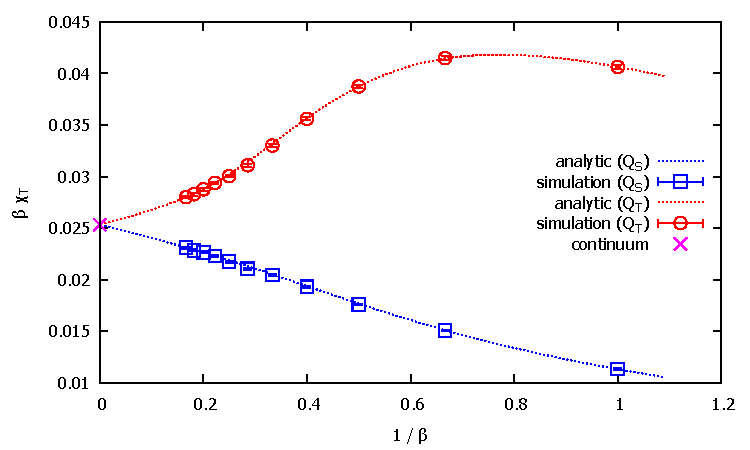
\includegraphics[width=1\textwidth]{figs/BeakDiagram}
  \caption{Quenched topological susceptibility.}
\end{figure}
%\end{frame}

%\begin{frame}{$F_\eta$ versus $F_\pi$}
  \begin{itemize}
    \item inserting the confirmed values for $m_\eta^2$
      and $\chi_T^{que}$ 
      \[
        F_{\eta}^2 = \frac{2N}{m_\eta^2}\chi_T^{que} =
          2N \left(\frac{\pi\beta}{N}\right)
          \left(\frac{1}{4\pi^2\beta}\right) =
          \frac{1}{2\pi}
      \]
    \item we can compare the two decay constants
      \[
        F_\pi \simeq 0.386 \quad \overset{?}{=} \quad F_{\eta} = 0.399
      \]
    \item in large $N_c$ QCD, to the order $1/N_c$
      \[
        F_{\eta'} = F_\pi
      \]
    \item in the Schwinger model nothing assures that this relation 
      holds  
  \end{itemize}
%\end{frame}

\acknowledgments{
This work was supported by the Faculty of Geotechnical Engineering (University
of Zagreb, Croatia) through project "Change of the Eigenvalue Distribution at
the Temperature Transition" (2186-73-13-19-11).
??? Jaime and Wolfgang ???


Code development and testing were performed at the cluster Isabella of the
Zagreb University Computing Centre (SRCE) and production runs were run at the
Instituto de Ciencias Nucleares.


We thank Stephan D\"urr and Christian Hoelbling for discussions.
}


\bibliographystyle{JHEP-mcite}
\bibliography{../ref/ref}

%\begin{thebibliography}{99}
%\bibitem{...}
%....
%
%\end{thebibliography}

\end{document}
